\documentclass[letterpaper,12pt,addpoints]{exam}
\usepackage{amsmath}
\usepackage{bbm}
\usepackage{amssymb}
\usepackage[ruled,vlined]{algorithm2e}
\usepackage{xcolor}
\usepackage{hyperref}
\usepackage[shortlabels]{enumitem}
\usepackage{bm}
\usepackage{graphicx}

\DeclareMathOperator*{\argmin}{arg\,min}

% Declare Operators
\newcommand{\wv}{\mathbf{w}}
\newcommand{\bias}{b}
\newcommand{\xv}{\mathbf{x}}
\newcommand{\slack}{\xi}
\newcommand{\const}{C}
\newcommand{\margin}{M}
\newcommand{\kernel}{K}
\newcommand{\kernelmap}{\phi}
\newcommand{\param}{\gamma}
\newcommand{\st}{\mathop{\mathrm{subject\,\,to}}}

\newcommand{\ns}[1]{{\color{red}\bf NS: #1}}

\renewcommand\questionlabel{\thequestion)} %replace period with parenthesis
\renewcommand{\thequestion}{\bfseries\large\arabic{question}}

\newcommand\stoplabeling{\def\makelabel##1{}}
\newcommand\resumelabeling{\def\makelabel##1{\hss\llap{##1}}}
\nopointsinmargin
\pointformat{}

\usepackage[utf8]{inputenc}

\title{10-715 Fall 2020 Homeworks}

\begin{document}


\begin{center}
{\Large CMU 10-715: Midterm Exam}\\
{\bf DUE: Oct. 8, 2020, 11:40 AM Eastern time}.\\
\end{center}

\textbf{\large Instructions}:

\begin{itemize}
    \item It is a 24-hour exam. The submission site will close at 11:40 AM, Oct 8.

    \item You can refer to your own notes, the scribe notes, homework solutions, the text book, and lecture videos. You are \textbf{NOT} allowed to use any other resources (e.g., no searching on the Internet).
    
    \item You are \textbf{NOT} allowed to discuss the exam with anyone in the duration of the exam. For any questions, please post on Diderot.
    
    \item For the programming question(s), you can feel free to use any code you wrote for any of the homeworks. 
    
    \item Submit your solutions in a pdf file to Gradescope. Handwritten or typed solutions are both accepted. Start \textbf{each question on a new} page and make sure you select the corresponding page(s) for each question during submission to Gradescope. 
    
    \item We recommend taking a brief look at all questions first and then starting to answer them. You may find some questions easier than others. Good luck!
\end{itemize}

\begin{center}
\textbf{Distribution of Marks}\\
\medskip
\gradetable[v][questions]
\end{center}

\newpage
\begin{questions}
\question[10]
\section*{Enthusiastic Data Augmentation [10 pts]}
This is a ``conceptual'' question. You don't need to give formal proofs. Giving a text-based description, examples and/or pictures is fine.

\vspace{5mm}
Consider binary classification, with ${\cal{X}} = \mathbb{R}^d$ for some $d \geq 2$ and ${\cal Y} = \{-1,1\}$ and a  training dataset $\{(\xv_i,y_i)\}_{i \in [n]}$.


An enthusiastic student tries the following new approach towards training.
\begin{itemize}
    \item The student creates a new training dataset of $nd$ samples as follows.\\
    For each $i \in [n]$ and $j \in [d]$ define $\mathbf{z}_{ij} \in \mathbb{R}^{nd}$ whose $j^{th}$ coordinate equals the $j^{th}$ coordinate of $\xv_i$ and all other coordinates are zero. The following figure shows an example:\\
    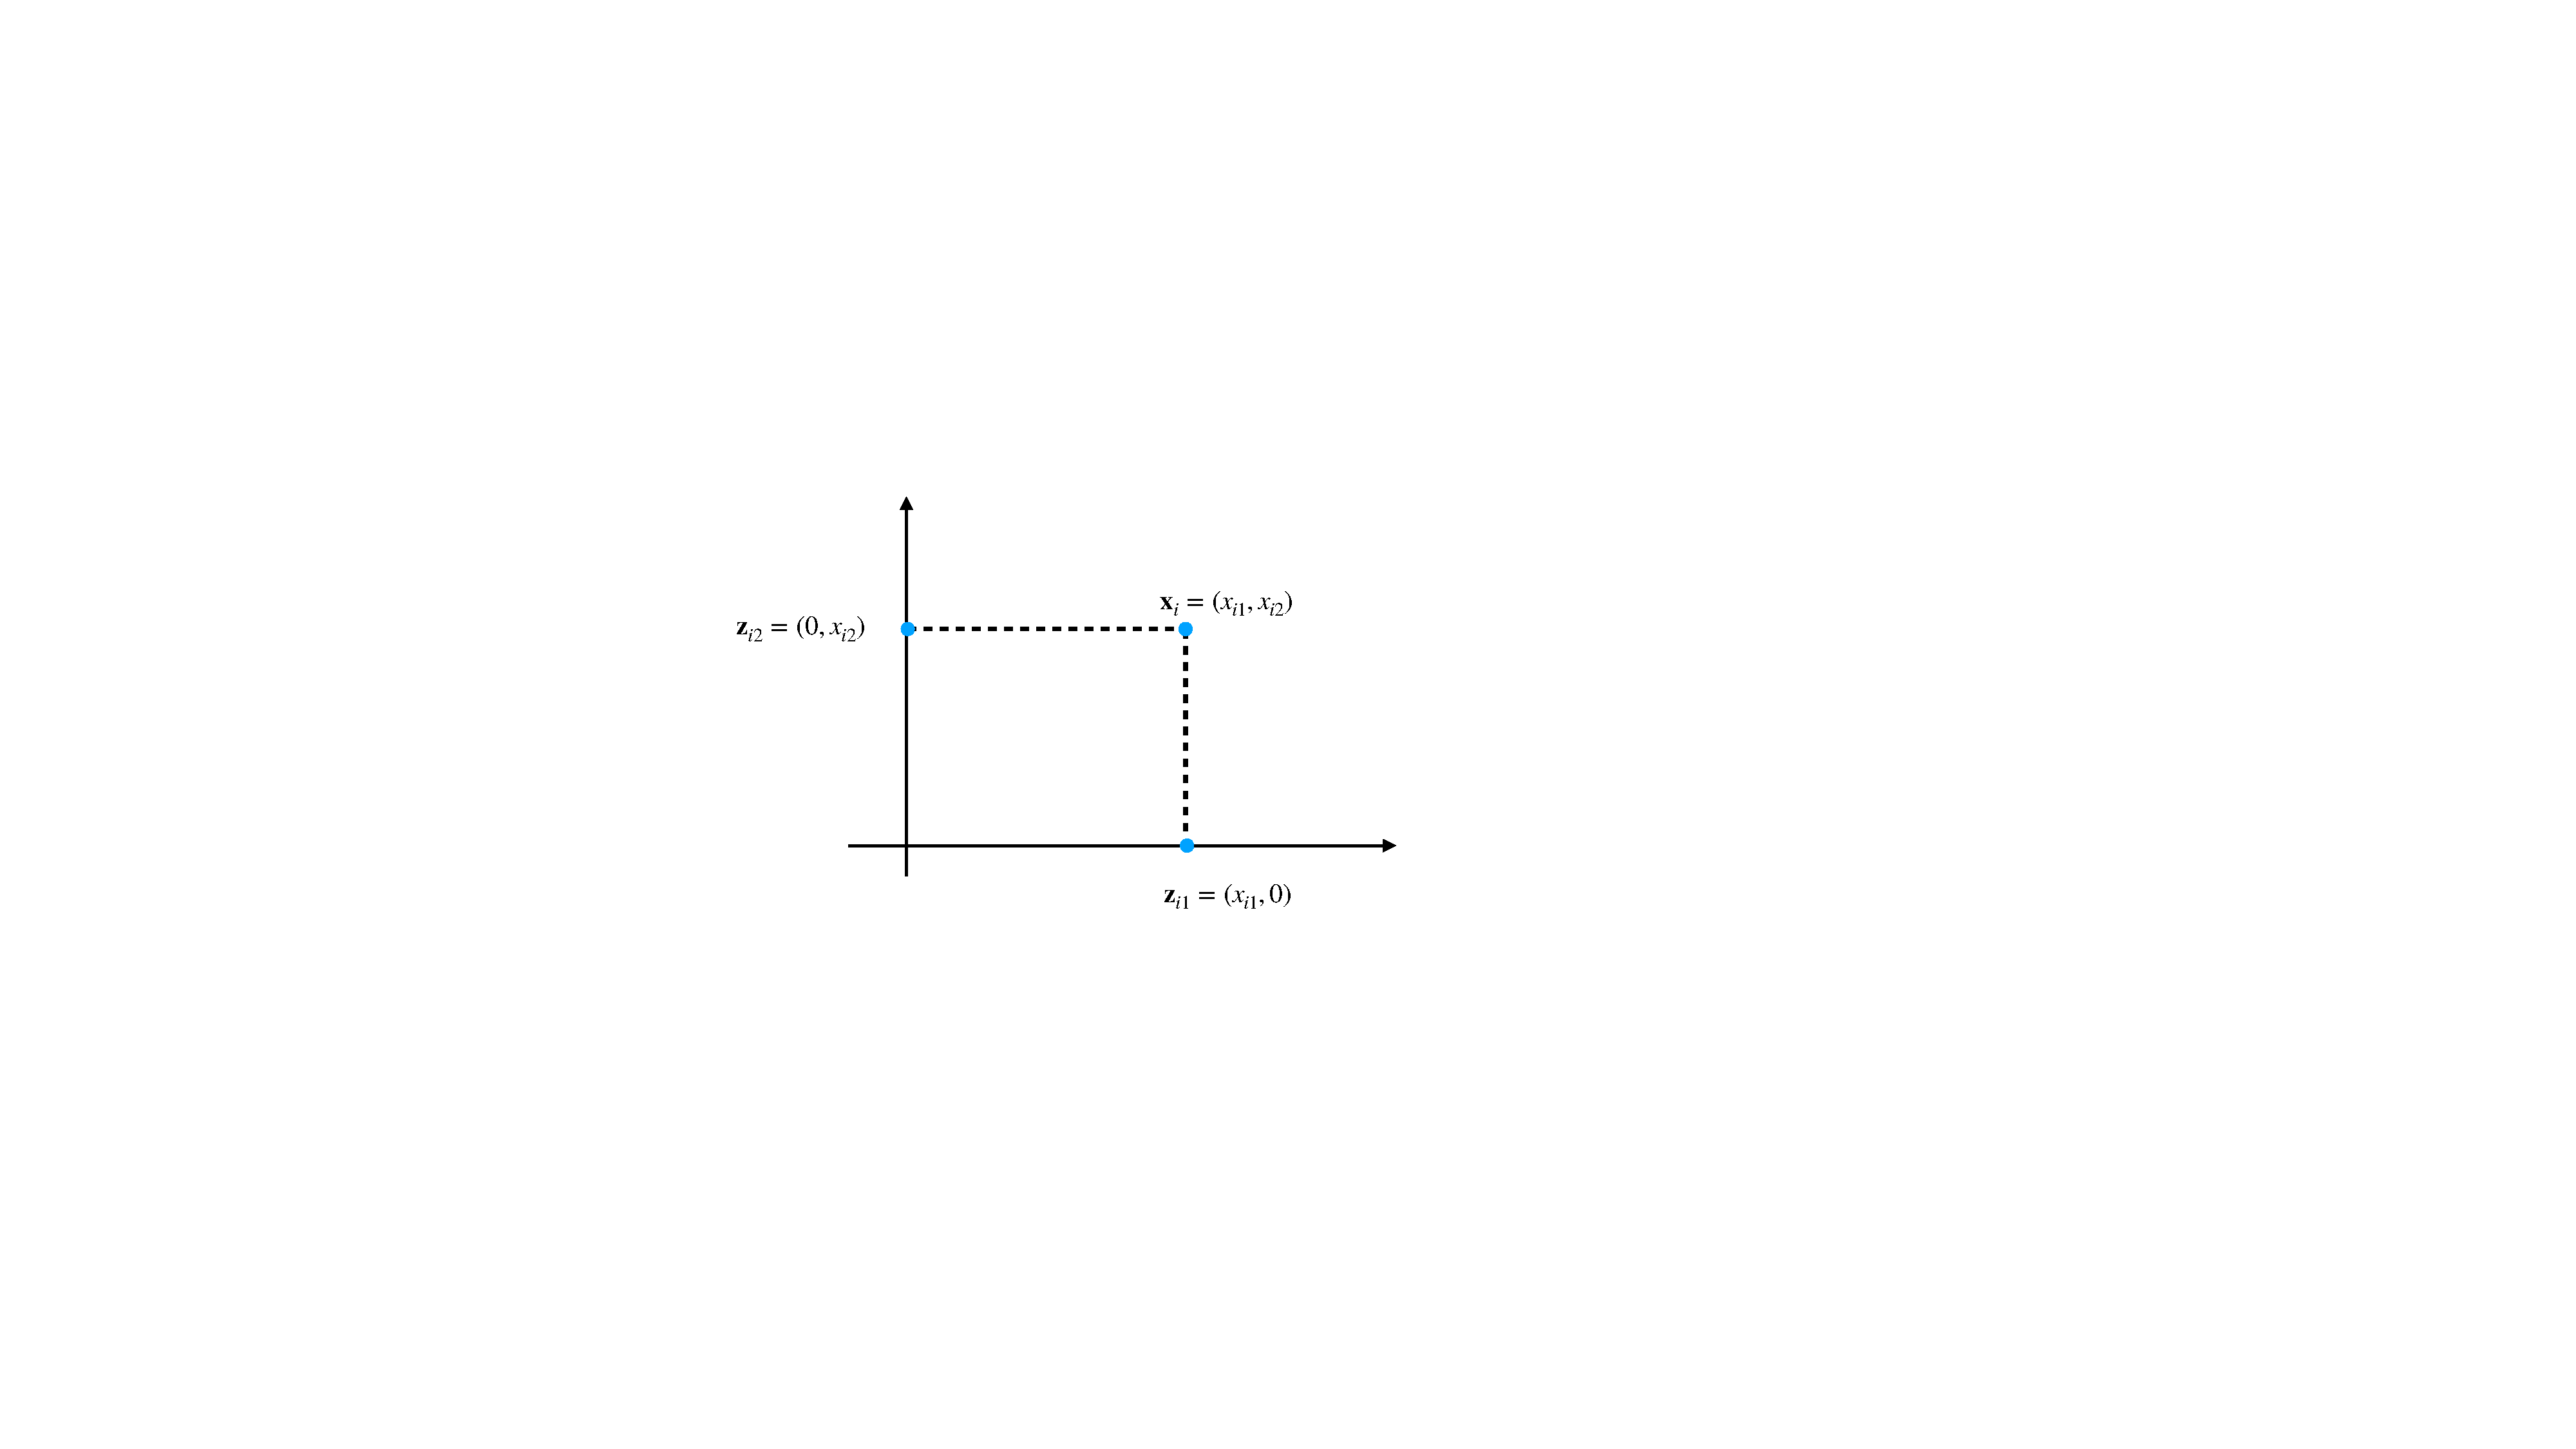
\includegraphics[width=0.5\linewidth]{midterm/images/enthusiastic.pdf}
    
     Now consider the modified training dataset:  $\{(\mathbf{z}_{ij},y_{ij})\}_{i\in [\,n\,]\; j\in [\,d\,]}$.

    \item The enthusiastic student trains a perceptron on this modified training set and obtains $\wv \in \mathbb{R}^d, b \in \mathbb{R}$.
    \item Given a new point $\xv \in \mathbb{R}^d$, the prediction is $f(\xv) = \text{sign} (\langle \wv, \xv \rangle + b)$.
\end{itemize}

\vspace{10mm}

What do you think about this idea? Are there settings where the perceptron algorithm can classify the original training data perfectly, but fails to do so on the modified training data? 


\addpoints

\newpage
\question
\section*{Perceptron on Non Linearly Separable Data [10 pts]}
Consider a binary classification problem, with ${\cal{X}} = \mathbb{R}^d$ and ${\cal Y} = \{-1,1\}$ and a  training dataset $\{(\xv_i,y_i)\}_{i \in [n]}$. Consider the perceptron algorithm seen in class. \\

\begin{algorithm}[H]
\SetAlgoLined
Initialize parameters $\mathbf{w}_{0}=0$, $b_{0}=0$, step $t=0$\;
 \While{$\exists i\in [n]$ such that $y_{i}(\mathbf{w}^\top \mathbf{x}_{i} + b)\leq 0$}{
   $\mathbf{w}_{t+1}=\mathbf{w}_{t}+y_{i}\mathbf{x}_{i}$\;
   $b_{t+1}=b_{t}+y_{i}$\;
   $t=t+1$\;
 }
 Output $\mathbf{w}_t$ and $b_t$
 \caption{Perceptron algorithm}
\end{algorithm} 

\vspace{5mm}

\begin{parts}
\part[5](5 pts) With this context, what does it mean for a training dataset $\{(\xv_i,y_i)\}_{i \in [n]}$ to not be linearly separable in terms of $\wv$ and $b$? Please write down the formal mathematical meaning of it.

\part[5] (5 pts) Prove or give a counter example: The perceptron algorithm  will never terminate when the training data is not linearly separable.
\end{parts}


\newpage
\question
\section*{Kernel Soft SVM implementation [25 pts]}

Consider the soft SVM objective:
\begin{equation}
\label{soft_svm_primal}
\begin{aligned}
& \underset{\wv, \xi_i}{\text{minimize}} && \frac{1}{2}||\wv||_2^2 + C\sum_{i=1}^n\xi_i\\
& \text{subject to} && y_i(\wv^T\psi(x_i) + b) \geq 1-\xi_i & i = 1,\ldots, n\\
& && \xi_i \geq 0 & i = 1,\ldots, n
\end{aligned}
\end{equation}

Equation \ref{soft_svm_primal} has its dual form:
\begin{equation}
\label{soft_svm_dual}
\begin{aligned} 
  & \underset{\alpha}{\text{maximize}} && \mathbf{1}^T\alpha - \frac{1}{2}\alpha^T \tilde{K}\alpha \\
  & \text{subject to} && 0\leq \alpha_i\leq C \; \text{for all } i, \quad \alpha^Ty = 0\\
\end{aligned}
\end{equation}
where $\alpha$ is the dual variable, $K_{ij} = \langle\psi(x_i), \psi(x_j)\rangle$, and $\tilde{K}_{ij} = y_iy_jK_{ij}$.

\vspace{5 mm}
In this question you will implement your own Kernel Soft SVM and test it on the data \textcolor{blue}{data.txt}\footnote{The data is provided to you on this link \url{https://github.com/ShenghaoWu/10715/midterm/}} using the CVXOPT library \url{https://cvxopt.org/}.

You should use the Radial Basis Function kernel:
$$\langle \psi(x_i), \psi(x_j) \rangle = K_{ij} = \exp\left(-\gamma||x_i - x_j||_2^2\right)$$



You are not allowed to use packages that directly implement the kernel SVM algorithm. Please append your code to the end of your pdf submission. Your code will \textbf{NOT} be evaluated by the Autograder.

\vspace{5mm}

\begin{parts}
\part[5] (5 pts) The quadratic programming solver method from CVXOPT \textcolor{blue}{solvers.qp()} uses as input the matrices $\mathbf{Q}, \mathbf{p}, \mathbf{G}, \mathbf{h}, \mathbf{A}, \mathbf{b}$.\footnote{Documentation: \url{https://cvxopt.org/userguide/coneprog.html\#quadratic-programming}.\\The $\preccurlyeq$ symbol represents componentwise inequality.} Write the correspondence between these inputs and the matrices of Equation \ref{soft_svm_dual}. 
\part[20] (20 pts) Fit the classifier with $\gamma = \{ 4, 100\}$ and $C=1$ on the training data using CVXOPT. 
After you fit your classifier, plot the original data and the decision boundaries for $\gamma = \{ 4, 100\}.$ You can use the python function \textcolor{blue}{contourf} on a fine meshgrid to plot the decision boundary.
\end{parts}

\newpage
\question[10]
\section*{Kernelizable Objectives and  the Representer Theorem [10 pts] }
Recall the Representer Theorem (and assume it as a given). Let $\psi:\cal X \rightarrow \cal F$ where $\cal F$ is Hilbert space. Consider $f : \mathbb{R}^n \rightarrow \mathbb{R}$. Now, there are many algorithms which optimize over the squared norm $||\mathbf{w}||^2$. Moreover, when trying to write down some algorithms in the form required by Mercer's theorem, they have some other function of $\mathbf{x_i}$'s as well in their objective. With this motivation, your goal is to prove that algorithms that optimize  the following objective are also kernelizable:

\begin{equation*}
    \argmin_{\mathbf{w} \in \cal F}~~~ f(\langle \mathbf{w}, \psi(\mathbf{x_1}) \rangle,..., \langle \mathbf{w}, \psi(\mathbf{x_n}) \rangle) + \tilde{R}(||\mathbf{w}||,||\mathbf{w}||^2) + g(\mathbf{x_1},...,\mathbf{x_n}).
\end{equation*}
 where $f(\langle \mathbf{w}, \psi(\mathbf{x_1}) \rangle,..., \langle \mathbf{w}, \psi(\mathbf{x_n}) \rangle)$ and $g(\mathbf{x_1},...,\mathbf{x_n})$ are arbitrary functions, $\tilde{R}(||\mathbf{w}||,||\mathbf{w}||^2)$ is coordinatewise non-decreasing.


\addpoints

\newpage
\question[10]
\section*{Validity of a Kernel [10 pts]}
Consider ${\cal X}=\mathbb{R}^d$ for some $d \geq 2$. Consider the function $K: {\cal X} \times {\cal X} \rightarrow \mathbb{R}$ as:
$$K(\mathbf{x},\tilde{\mathbf{x}}) = \log \left(\frac{1}{d}\right), \; \text{for all }  \mathbf{x},\tilde{\mathbf{x}} \in \mathcal{X}$$ 

Prove or disprove: $K$ is a valid kernel.

\addpoints

\newpage
\question[15]
\section*{Epsilon-net Arguments [15 pts]}
Although the epsilon-net argument works in many other problems, \textcolor{red}{here it does not} --- there are flaws in the arguments below. Your goal is to identify any one of the five steps below which does NOT work and justify your answer.  To be clear, you do not have to show whether other steps work or not -- just need to identify one step and show that the claim in that step is false.
\vspace{5mm}

Consider the realizability and i.i.d. assummptions. In the lecture, we proved a bound on the sample complexity of PAC learning when the hypothesis class ${\cal H}$ is a finite-sized class. In particular, we showed that ${\cal H}$ is $(\epsilon,\delta)$-PAC learnable as long as the number of samples is at least $\left \lceil{\frac{log(|\cal H|/\delta)}{\epsilon}}\right \rceil $. However, if the class ${\cal H}$ is infinite-sized, then however simple this class may be, simply substituting it in the bound above gives a vaccuous result. 

A common trick for using such results for finite settings in order to get results for infinite settings is called `epsilon-net arguments'. The high-level idea is to (i) quantize the infinite setting to obtain a finite setting, (ii) use the finite result, and (iii) show that the quantization doesn't hurt too much. 

Let us try that approach here.\\
Consider $\mathcal{X} = [0,1]$ and $\mathcal{H} = \{ h(x) = \text{sign}(x-\beta) | \beta \in [0,1]\}$. Clearly, $|\mathcal{H}|=\infty$. The goal is to use the above PAC learning result (which was derived for finite-sized $\mathcal{H}$) to obtain PAC learnability for this class via an epsilon-net argument.
\begin{enumerate}
    \item For some (finite) positive integer $k$, define $\mathcal{H}_k$ as the hypotheses have thresholds $0, 1/k, 2/k, ..., 1$, that is, $\mathcal{H}_k = \{ h(x) = \text{sign}(x-\beta) | \beta \in \{0, 1/k, 2/k, ..., 1\}\}$. Thus we have  $\mathcal{H}_k \subseteq \mathcal{H}$. 
    \item Since $|\mathcal{H}_k|=k+1 < \infty$, we can use the aforementioned result to get a sufficient sample size for $(\epsilon/2,\delta)$-PAC learnability of ${\mathcal{H}_k}$ as   $\left \lceil{\frac{2 \log((k+1)/\delta)}{\epsilon}}\right \rceil $.
    \item We can then show that there exists a large enough finite value of $k$ such that for every $h^* \in \mathcal{H}$, there exists some $h_k \in \mathcal{H}_k$ such that $R_{(D,h^*)}(h_k) \leq \epsilon/2$ for every distribution $D$. Denote this value of $k$ as $\xi$. 
    \item Finally consider the Empirical Risk Minizer (ERM) on class $\mathcal{H}_\xi$ and denote the output as $h_{ERM}$. Consider any true classifier $h^* \in \mathcal{H}$ and any distribution $D$. From point 3 above, let $h_{approx} \in \mathcal{H}_\xi$ be a hypothesis such that $R_{(D,h^*)}(h_{approx}) \leq \epsilon/2$. Show that $R_{(D,h^*)}(h_{ERM}) \leq R_{(D,h^*)}(h_{approx}) +     R_{(D,h_{approx})}(h_{ERM})$.
    \item Conclude that $\mathcal{H}$ is $(\epsilon,\delta)$-PAC learnable if the number of samples is at least\\ $\lceil \frac{2\log(|\mathcal{H}_{\xi}|/\delta)}{\epsilon} \rceil = \lceil\frac{2\log(|(\xi+1)|/\delta)}{\epsilon} \rceil$.
\end{enumerate}



\addpoints

\newpage
\question[15]
\section*{PAC Learnable [15 pts]}
Let a classification problem be defined by $\mathcal{X} = \mathbb{R}^d$ for some $d \geq 1$ and ${\cal Y} = \{-1,1\}$. \\
For any value of integer $m \geq 1$ and any $\mathbf{x_1},\ldots,\mathbf{x_m} \in \mathcal{X}$, define the hypothesis class:
\begin{align*}
    \mathcal{H}(\xv_1,\ldots,\xv_m) = \{ h: \mathcal{X} \rightarrow \mathcal{Y} \;|\; h(\xv_1) = \cdots = h(\xv_m) = 1, ~ \text{and } h(\xv)=-1 \text{ for other  } \xv \in \mathcal{X} \}.
\end{align*}
Now define,
\begin{align*}
    \mathcal{H}_m = \bigcup_{\xv_1,\ldots,\xv_m \in \mathcal{X}} \mathcal{H}(\xv_1,\ldots,\xv_m).
\end{align*}
Finally define,
\begin{align*}
    \mathcal{H} = \bigcup_{\text{all integers } m \geq 1} \mathcal{H}_m.
\end{align*}


Is the class $\mathcal{H}$ PAC learnable (under realizability)? If yes, derive an upper bound on its sample complexity. Supplement your responses with proofs.

\addpoints

\newpage
\question
\section*{No Free Lunch Theorem [15 pts]}
Consider any hypothesis class $\mathcal{H}$. 
\begin{parts}
\part[10] (10 pts) Recall the no free lunch theorem: If the sample size $n$ and the feature space $\cal X$ satisfy $n<\frac{|\cal X|}{2}$ then,
for any learning algorithm (whose output is denoted by $h$) it must be that 
$$\mathbb{P}(R(h)\geq \frac{1}{8})\geq \frac{1}{7}.$$

Use the statement of the no free lunch theorem to prove that if the VC dimension of $\mathcal{H}$ is infinite, then $\mathcal{H}$ is not PAC learnable under realizability.

\part[5] (5 pts) Prove that if  $\mathcal{H}$ is not PAC learnable under the realizability assumption then it is not agnostically PAC learnable.
\end{parts}

\end{questions}

\end{document}